\documentclass{article}
\usepackage{graphicx}
\usepackage[margin=1in]{geometry}
\usepackage{amsmath}
\title{Mathematical Modeling Project}
\author{Tyler Lukasiewicz, Liana Severo, Caitlin Buttery}
\begin{document}
\maketitle
\abstract{
babkabkaka mea quidam pericula appellantur, ne quo vitae recteque. Duo ullum deserunt definitiones ea, ex has vocent constituam inciderint, at novum philosophia has. Summo facete audire eu pro, mazim tritani tibique ne quo. Justo deterruisset reprehendunt qui cu, nam te debet oblique incorrupte. Usu nominavi copiosae patrioque et, nec ferri constituto ei.

}
\section{Introduction}
\label{sec:Introduction}
Lorem ipsum dolor sit amet, id mea quidam pericula appellantur, ne quo vitae recteque. Duo ullum deserunt definitiones ea, ex has vocent constituam inciderint, at novum philosophia has. Summo facete audire eu pro, mazim tritani tibique ne quo. Justo deterruisset reprehendunt qui cu, nam te debet oblique incorrupte. Usu nominavi copiosae patrioque et, nec ferri constituto ei.


\section{Research and Methods}
\label{sec:Main part}

\subsection{Immune System Response to a Single Viral Strain}
\begin{equation}
    \begin{cases}
        \dot v &= v(r-ax) = f_1(v,x), \\
        \dot x &= -bx + cv = f_2(v,x)
    \end{cases}
\end{equation}

Here, $v$ is the viral strain. $x$ is the specific immune system response to the strain. $r$ is the rate at which the virus reproduces. $a$ is the rate at which the immune cells destroy the virus. $b$ is the rate at which the immune cells die off. $c$ is rate at which the immune cells reproduce, which is dependent on the number of viruses present, $v$.  
\subsubsection{Getting our eigenvalues}
First we take the Jacobian matrix of our system, which is
\begin{equation}
    J =
    \begin{pmatrix}
        r-ax    & -av \\
        c       & -b
    \end{pmatrix}
\end{equation}
Then we find the characteristic equations by evaluating the Jacobian at the two fixed points of our system $(0,0)$ and $(\alpha,\beta)$, where $\alpha = \frac{br}{ac} $ and let $\beta = \frac{r}{a} $
\begin{equation}
    \begin{split}
        &J(0,0) - \lambda I = \lambda^2 + \lambda(b-r) -br = 0\\
        &\implies \lambda_{1,2} = r,-b\\
        &J(\alpha,\beta)  - \lambda I =  \lambda^2 + \lambda \gamma + \delta\\ 
        &\implies \lambda_{1,2} = \frac{-\gamma \pm \sqrt{\gamma^2 - 4\delta}}{2} \\
        \text{where} \\
        &\gamma =  b - r + a\beta \text{, and } \delta = ac\alpha + ab\beta -rb
    \end{split}
\end{equation}
\subsubsection{Modeling the System With One Viral Strain}
We will now model our system of equations with conditions $r = 2.4, a = 2, b = 0.1, \text{ and }c = 1.$. We will also assume that we are starting with no viruses and no immune response.
\label{sub:modeling the sytem}

The fixed point $(0,0)$ corresponds to the eigenvalues $\lambda_1 = 2.4, \lambda_2 = -.1$, which implies that $(0,0)$ is a saddle point. The fixed point $(\alpha,\beta) = (.12,1.2)$ results in eigenvalues $\lambda_1 = -.05 + 4.873i , \lambda_2 = -.05 - 4873i$, which implies that the point $(.12,1.2)$ is a spiral sink. So in this system both the viral strain and immune response will begin oscillating dramatically and then as time approaches infinity, they will settle to stable values. This is illustrated in figure \ref{fig:hiv1}
\label{sub:Determining Stability of Fixed points}
\begin{figure}[!tbp]
    \centering
    \begin{minipage}[b]{0.4\textwidth}
	    \caption{\textbf{\textit{Population sizes for a single virus strain with r = 2.4, a = 2, b = 0.1, c = 1.}}}
	    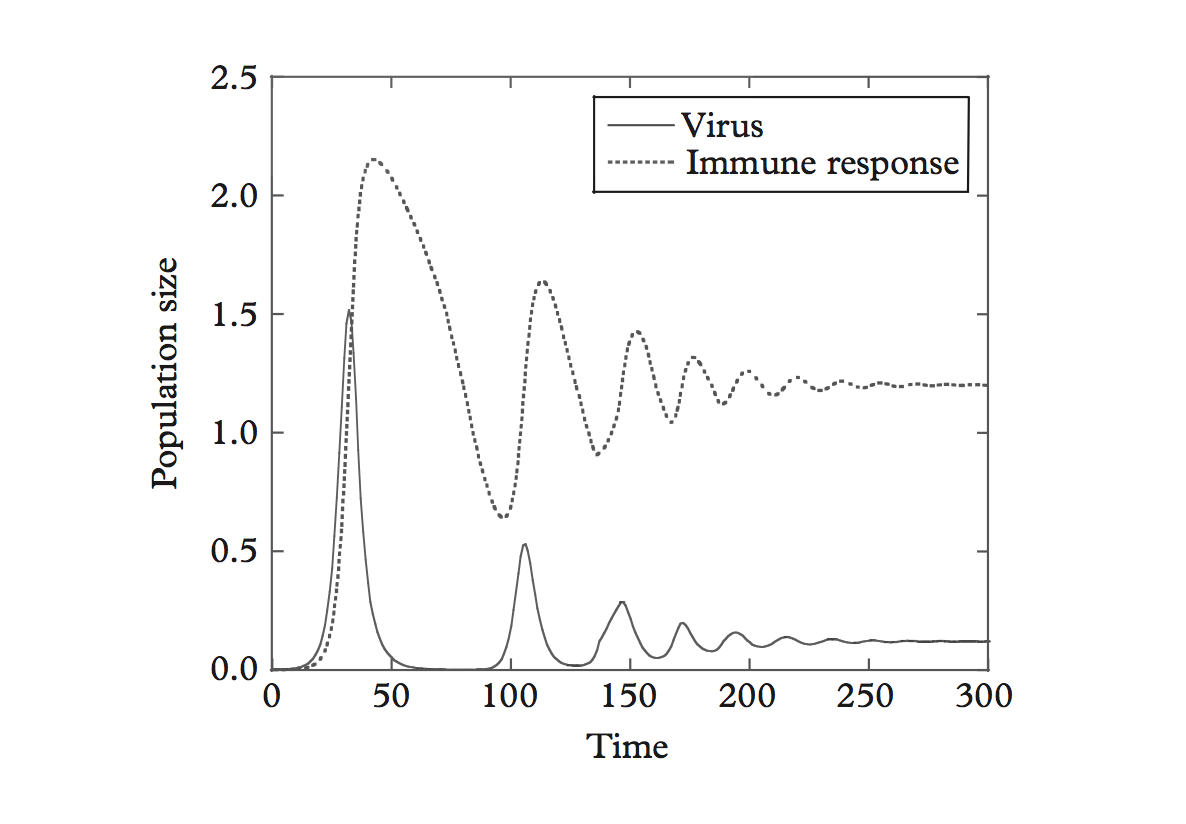
\includegraphics[scale=.25]{imgs/hiv_graph1.png}
	    \label{fig:hiv1}
	\end{minipage}
	\hfill
	\begin{minipage}[b]{0.4\textwidth}
		\caption{\textbf{\textit{Population sizes for multiple strains  with r = 2.4, a = 2, b=0.1,c=1,q=2.4,k=1.}}}
		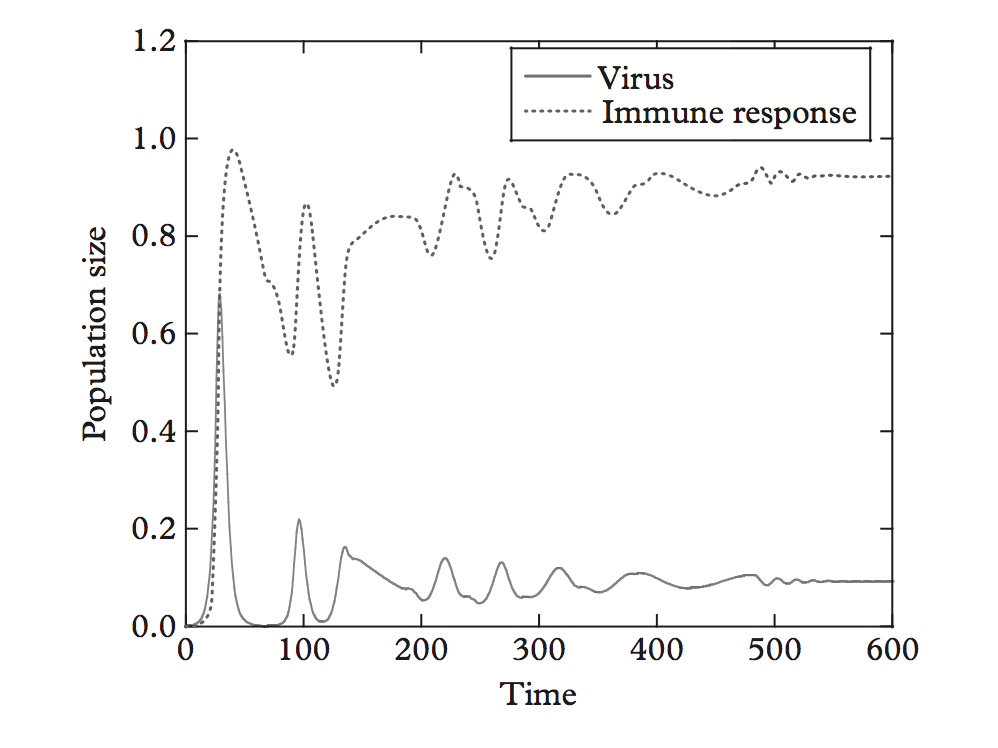
\includegraphics[scale=.25]{imgs/hiv_graph2.png}
		\label{fig:hiv2}
	\end{minipage}
\end{figure}

\subsection{Modeling the System with Multiple Viral Strains}
Suppose there are $N$ strains of the virus.  The $i$th strain of the virus $v_i$ and the immunal reaction $x_i$ to it can be modeled by the system of equations
\begin{equation}
    \begin{cases}
        \dot v_i &= v_i(r - ax_i), \\
        \dot x_i &= -bx_i + cv_i
    \end{cases}
\end{equation}
This adds a degree of randomness to our behavior, as new viruses can appear at any point in time. We may begin with only one virus, which can proceed to mutate as it pleases, or we may begin with many strains. Each new viral strain should result in a new immune response. Eventually, a global immune response will take care of all $N$ viral strains regardless of mutation or rate of mutation. This global response can be modeled by the system of equations
\begin{equation}
    \begin{cases}
        \dot v_i &= v_i(r - ax_i - qz) \\
        \dot x_i &= -bx_i + cv_i \\
        \dot z &= kv - bz
    \end{cases}
\end{equation}
Where $z$ is the cross reactive response that decays at rate $b$.  $v = \sum^{N}_{i=1} v_i$ is the total viral load. $q$ is the rate at which the virus evades the global response, and $k$ is the rate at which the global response grows in comparison to the number of preheat viral strains.


\subsubsection{Getting Eigenvalues}
\label{sec:hiv2_evals}
In this case we are going to be introducing a the variable:
\[
V = \sum_{i = 1}^N v_i
\]
We will assume that $V$ is constant at each iteration. Thus our new system of equations becomes 
\begin{equation}
	\begin{cases}
		\dot v &= v(r - ax - qz) \\
		\dot x &= -bx + cv \\
		\dot z &= kV - bz
	\end{cases}
\end{equation}
First we take the Jacobian of the system of equations. 
%the jacobian
\begin{equation}
    J=
    \begin{pmatrix}
        -ax-qz+r    &-va    &-qv    \\
        c           &-b     &0      \\
        0           &0       &-b
    \end{pmatrix}
\end{equation}
%the characteristic equation
Next we find the characteristic equation
\begin{equation}
    \begin{split}
        | J - \lambda I | &= \\ 
        &-a{b}^{2}x-abcv-2\,ab\lambda\,x-ac\lambda\,v-a{\lambda}^{2}x-{b}^{2}qz \\
        &-2\,b\lambda\,qz-{\lambda}^{2}qz-{b}^{2}\lambda+{b}^{2}r-2\,b{\lambda}^{2}+2\,b\lambda\,r-{\lambda}^{3}+{\lambda}^{2}r
    \end{split}
\end{equation}

solving for lambda, we get the eigenvalues

\begin{equation}
    \begin{split}
        \lambda_1 &=  -b\\
        \lambda_{2,3} &= -1/2\,ax-1/2\,qz-b/2+r/2 \\
        &\pm 1/2\,\sqrt {{a}^{2}{x}^{2}+2\,axqz+{q}^{2}{z}^{2}-2\,abx-4\,acv-2\,axr-2\,bqz-2\,qzr+{b}^{2}+2\,br+{r}^{2}}         
    \end{split}
\end{equation}


\subsubsection{Modeling The Equation}

We will be studying the behavior of this equation with the values

\begin{equation}
    \begin{split}
        r = 2.4, a = 2, b=0.1,c=1,q=2.4,k=1
    \end{split}
    \label{eq:vals}
\end{equation}

Our first step is to determine the fixed points of the system of equations. In this case there are two.

%fixed points of equation
\begin{equation}
	\begin{split}
		&\text{Fixed point 1: } \quad v=0,x=0,z={\frac {kV}{b}} \\
		&\text{Fixed point 2: } \quad v=-{\frac {qkV-br}{ac}},x=-{\frac {qkV-br}{ab}},z={\frac {kV}{b}} 
	\end{split}
	\label{eq:fixed}
\end{equation}

Our observations show that our first fixed point will act as a source and the second will act as a spiral sink. This is demonstrated in figure \ref{fig:hiv2}


\subsection{HIV Section}

Now we will shift our focus to HIV specifically. HIV, the precursor to AIDS, destroys the immune system so the body cannot fight back against any illness, viral or otherwise. It kills white blood cells (a specific type known as a CD4 cell) and makes copies of itself within said cell. This will use our same system as before with our multiple viral strains with two differences; this time, a damping term is introduced in our equations for our immune cell production and our global immune response equation, reflecting the destruction of the body’s immune cell production and the slowing of the global immune response, respectively.

\begin{equation}
	\begin{cases}
		\dot v_i &= v_i (r-ax_i-qz)\\
		\dot x_i &= -bx_i + cv_i - uvx_i\\
		\dot z &= kv - bz - uvz
	\end{cases}
\end{equation}

Once again we will be introduce the variable $V$ as defined in section \ref{sec:hiv2_evals}. Thus we have the new system of equations that we can study to observe the interactions between viruses and immune response in this scenario.

\begin{equation}
	\begin{cases}
		\dot v=& v \left( -ax-qz+r \right) \\
		\dot x=& -uVx-bx+cv \\
		\dot z=& -uVz+kV-bz
	\end{cases}
\end{equation}

\begin{figure}[!tbp]
	\centering
	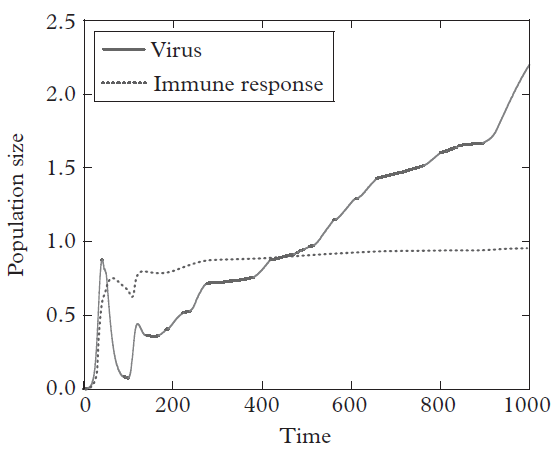
\includegraphics[scale=.5]{imgs/hiv_graph3.png}
	\caption{\textbf{\textit{The total population sizes of the
				viral load and the immune response with r = 2.4, a = 2, b = 0.1, c = 1,q = 2.4, k = 1, and u = 1}}}
	\label{fig:hiv3}
\end{figure}

\subsubsection{Identifying Eigenvalues}
As in previous sections our first step is to find the Jacobian
\begin{equation}
J = \left( \begin {array}{ccc} -ax-qz+r&-va&-vq\\ \noalign{\medskip}c&-Vu
-b&0\\ \noalign{\medskip}0&0&-Vu-b\end {array} \right) 
\end{equation}
From here we can evaluate our characteristic equation. 
\begin{equation}
	\begin{split}
		|J-\lambda I| &= -{V}^{2}a{u}^{2}x-{V}^{2}q{u}^{2}z-{V}^{2}\lambda\,{u}^{2}+{V}^{2}r{u}
		^{2}-2\,Vabux-Vacuv-2\,Va\lambda\,ux \\
		&-2\,Vbquz-2\,V\lambda\,quz-2\,Vb
		\lambda\,u+2\,Vbru-2\,V{\lambda}^{2}u+2\,V\lambda\,ru-a{b}^{2}x-abcv \\
		&-2\,ab\lambda\,x-ac\lambda\,v-a{\lambda}^{2}x-{b}^{2}qz-2\,b\lambda\,qz-
		{\lambda}^{2}qz-{b}^{2}\lambda+{b}^{2}r-2\,b{\lambda}^{2}+2\,b\lambda
		\,r-{\lambda}^{3}+{\lambda}^{2}r			
	\end{split}
\end{equation}

<<<<<<< HEAD
\section{Ebola Section}
=======
Finally, by solving our characteristic equation for $\lambda$ we can obtain our eigenvalues.

\begin{equation}
	\begin{split}
		\lambda_1 &= -Vu-b \\
		\lambda_{2,3} &= -1/2\,Vu-1/2\,ax-1/2\,qz-b/2+r/2 \pm 1/2\,\sqrt {\Phi}	\\
		\text{ where } \Phi  &= {V}^{2}{u}^{2}-2\,Vaux-2
		\,Vquz+{a}^{2}{x}^{2}+2\,axqz+{q}^{2}{z}^{2} \\
		&+2\,Vbu+2\,Vru-2\,abx-4\,c
		va-2\,arx-2\,bqz-2\,qzr+{b}^{2}+2\,br+{r}^{2}		
	\end{split}
\end{equation}

\subsubsection{Modeling The Equation}
We now present a model of the this system of equation with the following values:
\begin{equation}
a=2,b= 0.1,c=1,k=1,q= 2.4,r= 2.4,u=1
\end{equation}
At the following stable nodes:
\begin{equation}
\begin{split}
&\text{Fixed point 1: } \quad v=0,x=0,z={\frac {kV}{Vu+b}}   \\
&\text{Fixed point 2: } \quad  v=-{\frac {qkV-Vru-br}{ac}},x=-{\frac {qkV-Vru-br}{a \left( Vu+b \right) }},z={\frac {kV}{Vu+b}}
\end{split}
\label{eq:fixed}
\end{equation}
In this case, our virus will continue to grow as our immune system response stabilizes. Thus the host will die. 
%fixed points of equation
This is demonstrated in figure \ref{fig:hiv3}.

\subsection{Ebola Section}
>>>>>>> kablaa/master
Ebola is known to evade the immune system and go undetected during infection. We present a mathematical model done by Thomas Wester from the U.S. Naval Academy, using a system of non-linear ordinary differential equations derived from known biological dynamics and a few biologically reasonable assumptions.

\subsection{Biological Background}
Ebola is one of the deadliest viruses currently known to man and has resulted in several thousand cases and deaths as of recently, especially in epidemics happening in Africa and other highly impacted places. The Ebola virus produces one of the most lethal forms of hemorrhagic fever. As a result, the virus maintains mortality rates between 40\% and 90\%, averaging about 50\% and can cause death in less than two days, according to research done by Wester.\\
\\
Prior to the development of the mathematical model, it is crucial to understand how the human immune system responds to viral infections. Survival from Ebola virus highly depends on the host's ability to develop and manifest a strong response early after the introduction of the virus. A primary component of the immune system is the T-cell which has a lymphocyte. T-cell activation is one of the central events in the initiation of an adaptive immune response. There are two distinct populations of T-cells - Helper T-cells and Cytotoxic T-lymphocytes (from here on out referred to a CTLs) - and upon undergoing several binding events, the Helper T-cells and CTLs become activated.\\
Activated Helper T-cells serve as the alarm system of the immune system, which aids in the activation and proliferation of CTLs, which possess the ability to kill the infected cell that the Helper T-cells identify as harmful.\\
The main point to get from this is that CTL activation is the central event in the initiation of the immune system response and crucial for host survival and recovery. In Wester's research paper, he expands on analysis by considering CTL response to the introduction of the virus as well as the ability of the Ebola virus to evade detection by the host immune system.

\subsection{The Herz Model}
The Herz Model is a deterministic model for viral reproduction, which describes all events using a system of three equations:\\
\\
	x(t) = number of uninfected cells\\
	y(t) = number of infected cells\\
	v(t) = number of free virus particles\\
\\
And a modification, since contact between a virus and a cell reduces the number of available free virus.

\begin{equation}
		\dot x = \lambda - \mu x - \beta vx\\
\end{equation}
\begin{equation}
		\dot y = \beta vx - \alpha y\\
\end{equation}
\begin{equation}
		\dot v' = cy - \gamma v\\
\end{equation}
\begin{equation}
		\dot v = cy - \gamma v - \beta vx\\
\end{equation}

In equation (13), $\lambda$, $\mu$, and $\beta$ are the supply, death, and virus infection rates of uninfected cells, respectively.
In equation (14), $\alpha$ is the natural death rate of infected cells.
In equation (15), c is the rate at which infected cells produce virus, and $\gamma$ is the natural attrition of free virus particles.\\


\subsection{Ebola Application of the Herz Model}
Wester's model considers four distinct populations which are denoted:\\
\\
X(t): density of uninfected cells at time t,\\
I(t): density of infected cells at time t,\\
V(t): density of virus at time t,\\
T(t): density of CTL cells at time t.\\
\\
Thus, we consider the mathematical model of Ebola virus infection with an immune response given by the following 4-dimensional non-linear system of ordinary differential equations:

\begin{equation}
\begin{split}
	\dot X &= \lambda - \mu X(t) - \beta V(t)X(t) \\
	\dot I &= \beta V(t)X(t) - \rho I(t)T(t) - \alpha I(t) \\
	\dot V &= cI(t) - \gamma V(t) \\
	\dot T &= \rho I(t)T(t) - \delta T(t) \\
\end{split}
\end{equation}

With initial conditions X(0) = $X_{0}$, I(0) = $I_{0}$, V(0) = $V_{0}$, T(0) = $T_{0}$, and parameters $\lambda$ = growth rate of uninfected cells, $\mu$ = death rate of uninfected cells, $\beta$ = interaction rate of virus and uninfected cells, $\rho$ = interaction rate of infected cells and CTLs, $\alpha$ = death rate of infected cells, c = growth rate of virus, $\gamma$ = death rate of virus, and $\delta$ = death rate of CTLs.

\subsection{Fixed Points (Equilibria)}

For the model we consider the equilibrium (fixed) point for the populations (X, I, V, T). At the equilibrium, the rate of change for each population is zero:

\begin{equation}
	\begin{split}
		\dot X &= 0 \\
		\dot I &= 0 \\
		\dot V &= 0 \\
		\dot T &= 0 \\
	\end{split}
\end{equation}

If the values for any population at the fixed point is zero, those cells are defined as extinct, meaning that at long times, the populations will cease to exist. Thus, if V = I = 0 at the fixed point, the virus is extinct from the body as t $\rightarrow$ $\infty$, and the fixed point is known are Viral Free equilibrium. However, if the value for any population at the fixed point is not zero, those cells are defined as persistent. Thus, if V $\neq$ 0 and I $\neq$ 0, then the virus persists and the fixed point is known as Viral Persistence equilibrium. In addition, if T $\neq$ 0, then the immune response persists as t $\rightarrow$ $\infty$ and the fixed point is known as Immune Persistence equilibrium.\\
\\
If the system takes on an equilibrium at any time, it will remain at the value for all remaining time; however, unless the initial conditions are exactly one of the fixed points, the system need not necessarily obtain these values. The system may approach the fixed point, move away from the fixed point, or cycle between specific fixed points. In order to accurately determine which type of behavior we will obtain, we perform a stability analysis by linearizing the system and thus calculating the Jacobian matrix, which provides a linear approximation, and that occurs at the fixed points, which will be denoted $P_{n}$ from here on out.\\
\\
Here we present the relevant fixed points, $P_{n}$ = (X, I, V, T) for n = 1, 2, 3:

\begin{equation}
	\begin{split}
		P_{1} &= (\frac{\lambda}{\mu}, 0, 0)\\	
		P_{2} &= (\frac{\alpha \gamma}{c \beta}, \frac{c  \beta \lambda - \alpha \gamma \mu}{c \alpha \beta}, \frac{c \beta \lambda - \alpha \gamma \mu}{\alpha \beta \gamma}, 0)\\
		P_{3} &= (\frac{\gamma \lambda \rho}{c \beta \delta + \gamma \mu \rho}, \frac{\delta}{\rho}, \frac{c \delta}{\gamma \rho}, \frac{-c \alpha \beta \gamma + c \beta \lambda \rho - \alpha \gamma \rho \mu}{\rho (c \beta \delta + \gamma \mu \rho)})\\
	\end{split}
\end{equation}

With $P_{1}$ being the Viral Free equilibrium, and $P_{2}$ and $P_{3}$ representing the Viral Persistence equilibrium.\\
\\
The Jacobian for the linearized system is:\\

\[J(X, I, V, T) =
	\begin{bmatrix}
		V \beta - \mu & 0 & -X \beta & 0 \\
		V \beta & \alpha - T \rho & X \beta & -I \rho \\
		0 & c & - \gamma & 0 \\
		0 & T \rho & 0 & - \delta + I \rho
	\end{bmatrix}
				\]\\

\subsection{Stability Analysis for $P_{1}$}

The Jacobian evaluated at $P_{1}$ = ($\frac{\lambda}{\mu}$, 0, 0, 0) becomes:

\[J_{1} =
	\begin{bmatrix}
		- \mu & 0 & - \frac{\beta \lambda}{\mu} & 0 \\
		0 & \alpha & \frac{\beta \lambda}{\mu} & 0 \\
		0 & c & - \gamma & 0 \\
		0 & 0 & 0 & - \delta
	\end{bmatrix}
\]\\

and its characteristic equation:

\begin{equation}
	- \frac{1}{\mu}(-x - \delta)(x + \mu)(-c \beta \lambda + x^2 \mu + x \alpha \mu + x \gamma \mu + \alpha \gamma \mu) = 0
\end{equation}

From the characteristic equation we can define:

\begin{equation}
	\begin{split}
		a_{1} &= \alpha + \gamma + \delta + \mu \\
		a_{2} &= \alpha (\gamma + \delta + \mu) - \frac{\beta c \lambda}{\mu} + \gamma (\delta + \mu) + \delta \mu \\
		a_{3} &= \frac{\mu (\alpha (\gamma (\delta + \mu) + \delta \mu) + \gamma \delta \mu ) - \beta c \lambda (\delta + \mu)}{\mu} \\
		a_{4} &= \alpha \gamma \delta \mu - \beta c \delta \lambda
	\end{split}
\end{equation}

such that

\begin{equation}
	- \frac{1}{\mu}(-x - \delta)(x + \mu)(-c \beta \lambda + x^2 \mu + x \alpha \mu + x\gamma \mu + \alpha \gamma \mu) = x^4 + a_{1}x^3 + a_{2}x^2 + a_{3}x + a_{4}
\end{equation}\\

Define:

\begin{equation}
	\begin{split}
		R_{0} &= \frac{c \beta \lambda}{\alpha \gamma \mu} \\
		R_{1} &= \frac{c \beta \lambda \rho}{\alpha (\gamma \rho \mu + c \beta \delta)}
	\end{split}
\end{equation}\\

to be reproductive constants of the system.\\
Biologically, $R_{0}$ represents the average number of infected cells produced by an initially infected cell over its lifetime. $R_{1}$ represents the number of infected cells that a single immune cell (CTL, in our case) is able to fight.

For the Viral Free Equilibrium ($P_{1}$), if $R_{0} < 1$, then $P_{1}$ is stable; however, if $R_{0} > 1$, then $P_{1}$ is unstable.\\
\\
\\Insert figure of phase portrait here
\\ Figure 1 illustrates the interaction between the virus and uninfected cell populations given that $R_{0}, R_{1} < 1$.

\subsection{Stability Analysis for $P_{2}$}

The Jacobian evaluated at $P_{2} = (\frac{\alpha \gamma}{c \beta}, \frac{c  \beta \lambda - \alpha \gamma \mu}{c \alpha \beta}, \frac{c \beta \lambda - \alpha \gamma \mu}{\alpha \beta \gamma}, 0)$ is:

\[J_{2} =
	\begin{bmatrix}
		- \mu - \frac{c \beta \lambda - \alpha \gamma \mu}{\alpha \gamma} & 0 & - \frac{\alpha \lambda}{c} & 0 \\
		\frac{c \beta \lambda - n\alpha \gamma \mu}{\alpha \gamma} & \alpha & \frac{\alpha \lambda}{c} & - \frac{(c \beta \lambda - \alpha \gamma \mu) \rho}{c \alpha \beta} \\
		0 & c & - \gamma & 0 \\
		0 & 0 & 0 & - \delta + \frac{(c \beta \lambda - \alpha \gamma \mu) \rho}{c \alpha \beta}
	\end{bmatrix}
\]\\

and its characteristic equation:

\begin{equation}
	- \frac{1}{c^2 \alpha^2 \beta \gamma^2}(c^2 \alpha(x + \alpha) \beta(-x - \gamma) \gamma(x \alpha \gamma + c \beta \lambda) - c(-cx \alpha^3 \beta \gamma^3 - c \alpha^3 \beta \gamma^3 \mu))(-x - \delta + \frac{(c \beta \lambda - \alpha \gamma \mu)\rho}{c \alpha \beta}) = 0
\end{equation}


$P_{2}$ is stable if and only if $R_{0} > 1$ and $R_{1} < 1$.\\

Insert Figure of viral phase portrait here: A viral phase portrait for $R_{0}$ = 2.1089 and $R_{1}$ = 0.84356.\\
Figure 2 illustrates the dynamic between the virus and uninfected cell populations given the values $R_{0} > 1$ and $R_{1} < 1$.

\subsection{Stability Analysis for $P_{3}$}

The Jacobian evaluated at $P_{3} = (\frac{\gamma \lambda \rho}{c \beta \delta + \gamma \mu \rho}, \frac{\delta}{\rho}, \frac{c \delta}{\gamma \rho}, \frac{-c \alpha \beta \gamma + c \beta \lambda \rho - \alpha \gamma \rho \mu}{\rho (c \beta \delta + \gamma \mu \rho)})$ is:

\[J_{2} =
	\begin{bmatrix}
		- \mu - \frac{c \beta \delta}{\rho \gamma} & 0 & - \frac{\beta \gamma \lambda \rho}{c \beta \delta + \gamma \rho \mu} & 0 \\
		\frac{c \beta \delta}{\rho \gamma} & \alpha - \frac{-c \alpha \beta \delta + c \beta \lambda \rho - \alpha \gamma \mu \rho}{c \beta \delta + \gamma \mu \rho} & \frac{\beta \gamma \lambda \rho}{c \beta \delta + \gamma \mu \rho} & - \delta \\
		0 & c & - \gamma & 0 \\
		0 & \frac{-c \alpha \beta \delta + c \beta \lambda \rho - \alpha \gamma \mu \rho}{c \beta \delta + \gamma \rho \mu} & 0 & 0
	\end{bmatrix}
\]\\

and its characteristic equation:

\begin{equation}
	- \frac{x(\beta c \gamma^2(\mu + x) - (\alpha + x)(\gamma + x)(\beta c \delta + \gamma \mu \rho)(\beta c \delta + \gamma \rho (\mu + x))) + \rho Y(\gamma + x)(\beta c \delta + \gamma \rho (\mu + x))(\alpha \gamma \mu \rho + \beta c(\alpha \delta - \lambda \rho))}{\gamma \rho(\beta c \delta + \gamma \mu \rho)} = 0
\end{equation}\\

If $R_{1} > 1$, $R_{0} > \frac{\delta}{\mu}$, $c \beta > \alpha \rho$, $\lambda (\gamma + \delta) > \alpha \delta^2$, then $P_{3}$ is stable.\\

Insert figure 3 here: A system phase portrait for $R_{0} = 4.6864$ and $R_{1} = 2.8119$.\\
Similar to figure 2, the virus population appears to approach zero several times during the course of infection, reaching very low levels within the system.


\section{Conclusion}
\label{sub:Conclusion}
Lorem ipsum dolor sit amet, id mea quidam pericula appellantur, ne quo vitae recteque. Duo ullum deserunt definitiones ea, ex has vocent constituam inciderint, at novum philosophia has. Summo facete audire eu pro, mazim tritani tibique ne quo. Justo deterruisset reprehendunt qui cu, nam te debet oblique incorrupte. Usu nominavi copiosae patrioque et, nec ferri constituto ei.



\begin{thebibliography}{9}
\bibitem{latexcompanion} 
Michel Goossens, Frank Mittelbach, and Alexander Samarin. 
\textit{The \LaTeX\ Companion}. 
Addison-Wesley, Reading, Massachusetts, 1993.



\end{thebibliography}


\end{document}
